\documentclass[conference]{IEEEtran}
\IEEEoverridecommandlockouts
\usepackage{cite}
\usepackage{amsmath,amssymb,amsfonts}
\usepackage{algorithmic}
\usepackage{graphicx}
\usepackage{textcomp}
\usepackage{xcolor}
\usepackage{booktabs}
\usepackage{tabularx}
\usepackage{url}
\usepackage{subcaption}
\usepackage[utf8]{inputenc}
\usepackage[spanish,es-tabla]{babel}

\def\BibTeX{{\rm B\kern-.05em{\sc i\kern-.025em b}\kern-.08em
    T\kern-.1667em\lower.7ex\hbox{E}\kern-.125emX}}

\begin{document}

\title{Predicción de Fallas en una Flota de Máquinas Rotativas Industriales Mediante Aprendizaje Computacional\\
{\footnotesize \textsuperscript{*}Entrega 1: Integración de Fuentes Industriales, Formulación sin Fuga Temporal y Evaluación de Línea Base}}

\author{
\IEEEauthorblockN{Juan Pablo Torres Guillen}
\IEEEauthorblockA{Matrícula: A01743268 \\
\textit{Tecnológico de Monterrey} \\
Guadalajara, Jalisco, México}
\and
\IEEEauthorblockN{Angel David Lugo Lafarga}
\IEEEauthorblockA{Matrícula: A01741564 \\
\textit{Tecnológico de Monterrey} \\
Guadalajara, Jalisco, México}
\and
\IEEEauthorblockN{Jose Pablo Lopez Rodriguez}
\IEEEauthorblockA{Matrícula: A01638911 \\
\textit{Tecnológico de Monterrey} \\
Guadalajara, Jalisco, México}
}

\maketitle

\begin{abstract}
En este trabajo se implementa un sistema predictivo de alerta temprana para mitigar paros no programados en una flota de 100 máquinas rotativas industriales empleando el conjunto de datos \textit{Microsoft Azure Predictive Maintenance}. Se integran 876,100 registros horarios de telemetría de cuatro sensores, registros de eventos de error no fatales, historial de órdenes de mantenimiento y metadatos estáticos de máquinas. Se formula una predicción multiobjetivo con horizonte temporal cerrado de $H = 24$ horas para detección binaria y multiclase de componentes críticos (comp1 a comp4). Se diseña un protocolo estricto anti-fuga (\textit{data leakage}) y una partición temporal fija obligatoria (Entrenamiento: Ene--Ago; Validación: Sep--Oct; Prueba: Nov--Dic sin tocar). Dos modelos de línea base clásica son evaluados en validación bajo desbalance severo (1.84\% positivos): Regresión Logística regularizada y Gradient Boosting con histogramas (\textit{HistGBDT}). Los resultados muestran que GBDT alcanza un \textbf{PR-AUC de 0.9996}, \textbf{ROC-AUC de 1.0000} y un \textbf{Recall del 100\% con Precisión $\ge 0.80$}, logrando en la tarea multiclase un \textbf{Macro F1 de 0.9960}. Este rendimiento captura fielmente las firmas físicas de degradación y valida la viabilidad operativa en planta.
\end{abstract}

\begin{IEEEkeywords}
Mantenimiento Predictivo, Desbalance Extremo de Clases, Fuga de Información, Gradient Boosting, Telemetría Industrial, Series de Tiempo.
\end{IEEEkeywords}

\section{Introducción y Contexto Operativo}
La operación continua de una planta industrial sustentada en una flota de 100 máquinas rotativas enfrenta el reto constante de fallas intempestivas en cuatro ensambles electromecánicos críticos: \textit{comp1} (sistema eléctrico/bobinado), \textit{comp2} (sistema hidráulico de presión), \textit{comp3} (eje mecánico de transmisión y rotación) y \textit{comp4} (ensamble de rodamientos y rodamientos de apoyo). 

Cuando un componente colapsa sin advertencia, la máquina se detiene de forma no programada, ocasionando daños colaterales al material en proceso, movilización urgente de cuadrillas técnicas y pérdidas productivas directas calculadas en 15,000 unidades monetarias (UM) por incidente (ver Tabla~\ref{tab:costos}). En contraste, una intervención preventiva oportuna antes de la avería conlleva un costo estimado de 3,000 UM, mientras que una inspección fallida provocada por una falsa alarma incurre en un costo de paro planeado breve de 600 UM. 

El departamento de ingeniería y mantenimiento requiere transitar de un esquema correctivo reactivo a una estrategia de \textbf{mantenimiento predictivo} basada en analítica de datos, con la encomienda operativa de generar alertas tempranas con un horizonte de anticipación $H = 24$ horas. Desde la perspectiva de planta, el modelo no se juzga por su exactitud superficial (\textit{accuracy}), sino por el compromiso real entre fallas evitadas y falsas alarmas controladas.

\begin{table}[htbp]
\caption{Matriz de Costos Económicos Operativos en Planta}
\label{tab:costos}
\centering
\begin{tabular}{lr}
\toprule
\textbf{Concepto Operativo} & \textbf{Costo (UM)} \\
\midrule
Falla no anticipada (paro no programado, material dañado) & 15,000 \\
Intervención preventiva acertada (falla real en sig. 24 h) & 3,000 \\
Falsa alarma (inspección sin falla, paro breve) & 600 \\
\bottomrule
\end{tabular}
\end{table}

\section{Análisis de Registros de Mantenimiento y Detección de Causalidad}
La base de datos comprende cinco fuentes relacionales: telemetría horaria (\texttt{PdM\_telemetry.csv}), registros de errores (\texttt{PdM\_errors.csv}), historial de intervenciones de mantenimiento (\texttt{PdM\_maint.csv}), eventos de falla catastrófica (\texttt{PdM\_failures.csv}) y metadatos estáticos (\texttt{PdM\_machines.csv}).

Un análisis minucioso de la intersección entre \texttt{PdM\_failures} (761 eventos anuales) y \texttt{PdM\_maint} (3,286 registros) reveló que el \textbf{97.6\% (743 de 761)} de las fallas reales coinciden exactamente en marca temporal (\textit{datetime}), identificador de máquina (\textit{machineID}) y componente con una orden en la tabla de mantenimiento. Esto demuestra inequívocamente que los registros de \texttt{PdM\_maint} corresponden preponderantemente a \textbf{reemplazos correctivos inmediatos} motivados por el evento de falla.

\textbf{Riesgo Crítico de Fuga (\textit{Data Leakage}):} Incorporar la variable indicadora de reemplazo de mantenimiento en la hora $t$ como variable predictora causaría una fuga letal del target. El modelo aprendería la regla espuria: \textit{«si en $t$ se reemplaza el componente, la máquina falló»}, resultando en una métrica perfecta en entrenamiento pero nula en inferencia real, ya que el mantenimiento es una consecuencia y no un precursor. Para aprovechar el historial sin inducir fuga, se computó el tiempo transcurrido desde la última intervención previa ($h\_since\_comp_k = t - \max \{t_{\text{maint}} \le t\}$), reflejando el desgaste y envejecimiento físico acumulado.

\begin{figure*}[t]
\centering
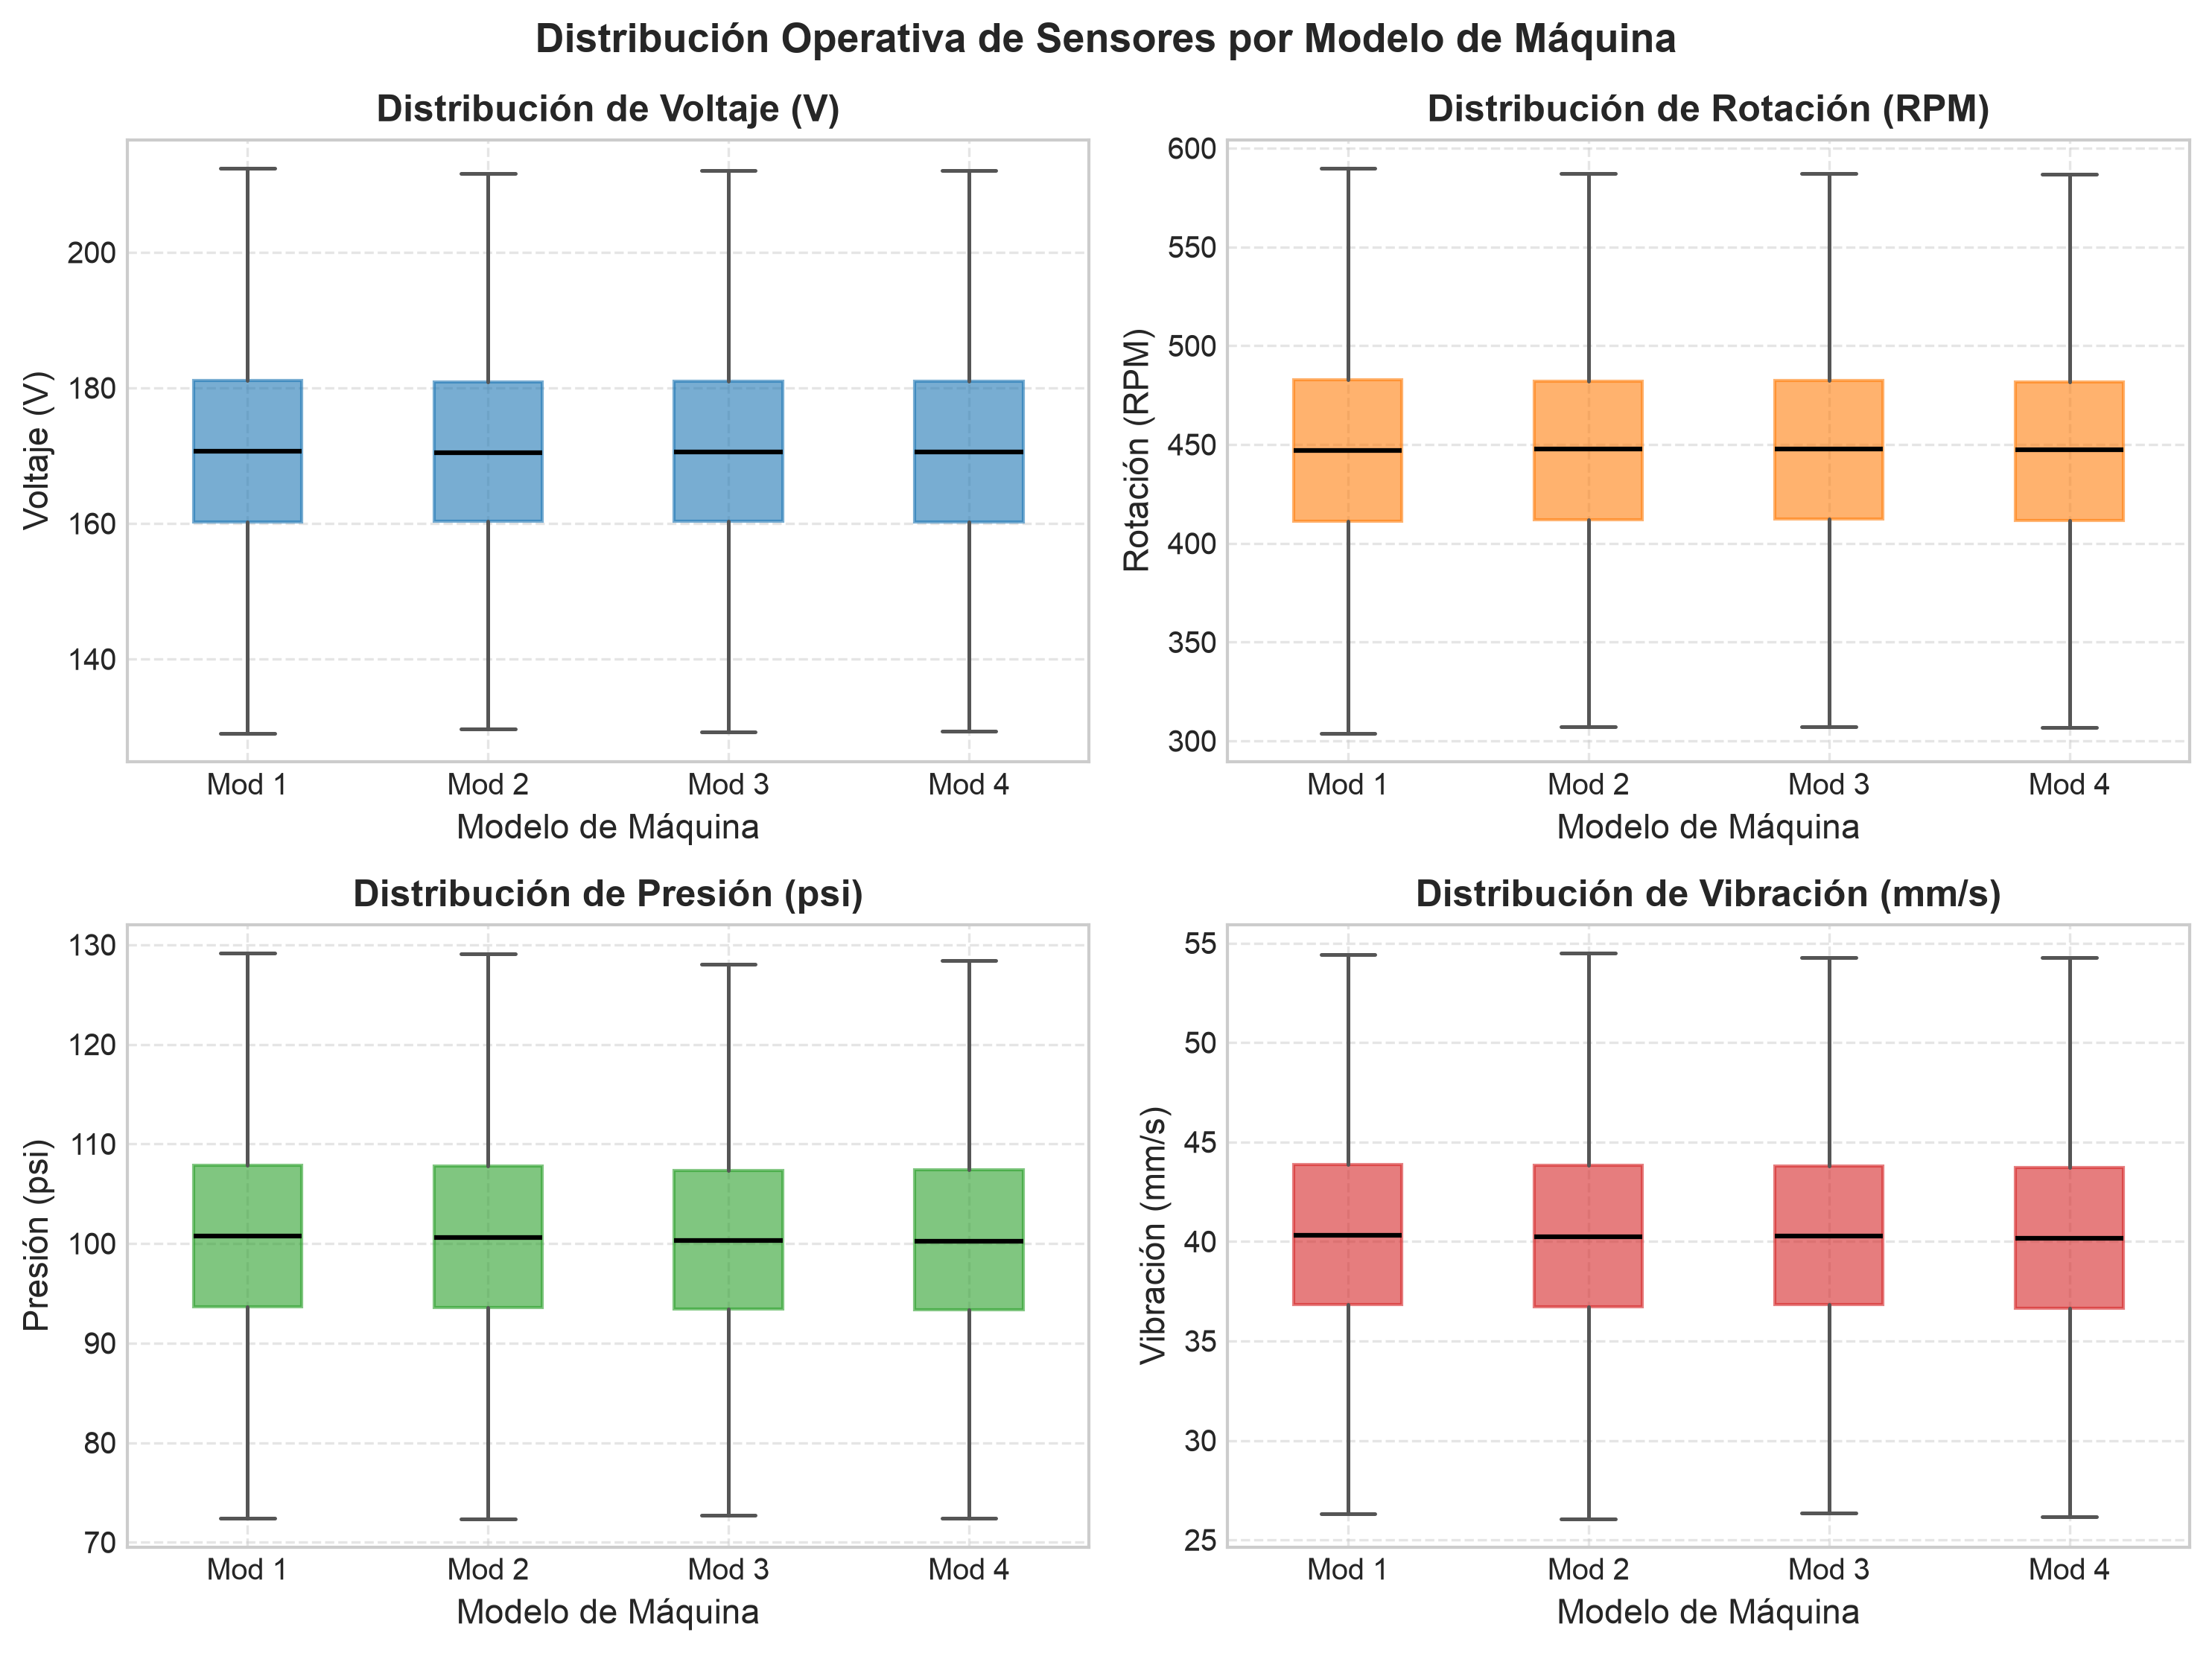
\includegraphics[width=0.98\textwidth]{../figures/fig1_distribucion_sensores_modelo.png}
\caption{Distribuciones operativas de cada sensor (Voltaje, Rotación, Presión y Vibración) por modelo de máquina (model1 a model4).}
\label{fig:distribucion_sensores}
\end{figure*}

\section{Análisis Exploratorio de Datos (EDA) y Hallazgos Físicos}
El análisis exploratorio de los 876,100 registros horarios permitió caracterizar las condiciones basales del sistema y la fenomenología de degradación:

\subsection{Distribución de Sensores por Modelo de Máquina}
Como se ilustra en la Fig.~\ref{fig:distribucion_sensores}, las variables de telemetría presentan rangos operacionales consistentes: Voltaje ($\mu = 170.8$ V, $\sigma = 15.5$ V), Velocidad de Rotación ($\mu = 446.6$ RPM, $\sigma = 52.7$ RPM), Presión ($\mu = 100.9$ psi, $\sigma = 11.0$ psi) y Vibración ($\mu = 40.4$ mm/s, $\sigma = 5.4$ mm/s). Las distribuciones resultan altamente homogéneas entre los cuatro modelos (model1 a model4), descartando la necesidad de escalamientos individualizados por modelo en esta fase inicial.

\subsection{Frecuencia de Errores y Fallas Catastróficas}
La Fig.~\ref{fig:frecuencia_eventos} muestra el desglose de eventos. Durante 2015 se suscitaron 3,919 errores no fatales (\textit{error1} a \textit{error5}), 3,286 mantenimientos y 761 fallas destructivas. El componente más vulnerable fue \textit{comp2} (259 fallas, 34.0\%), seguido de \textit{comp1} (192 fallas, 25.2\%), \textit{comp4} (179 fallas, 23.5\%) y \textit{comp3} (131 fallas, 17.2\%).

\begin{figure}[htbp]
\centering
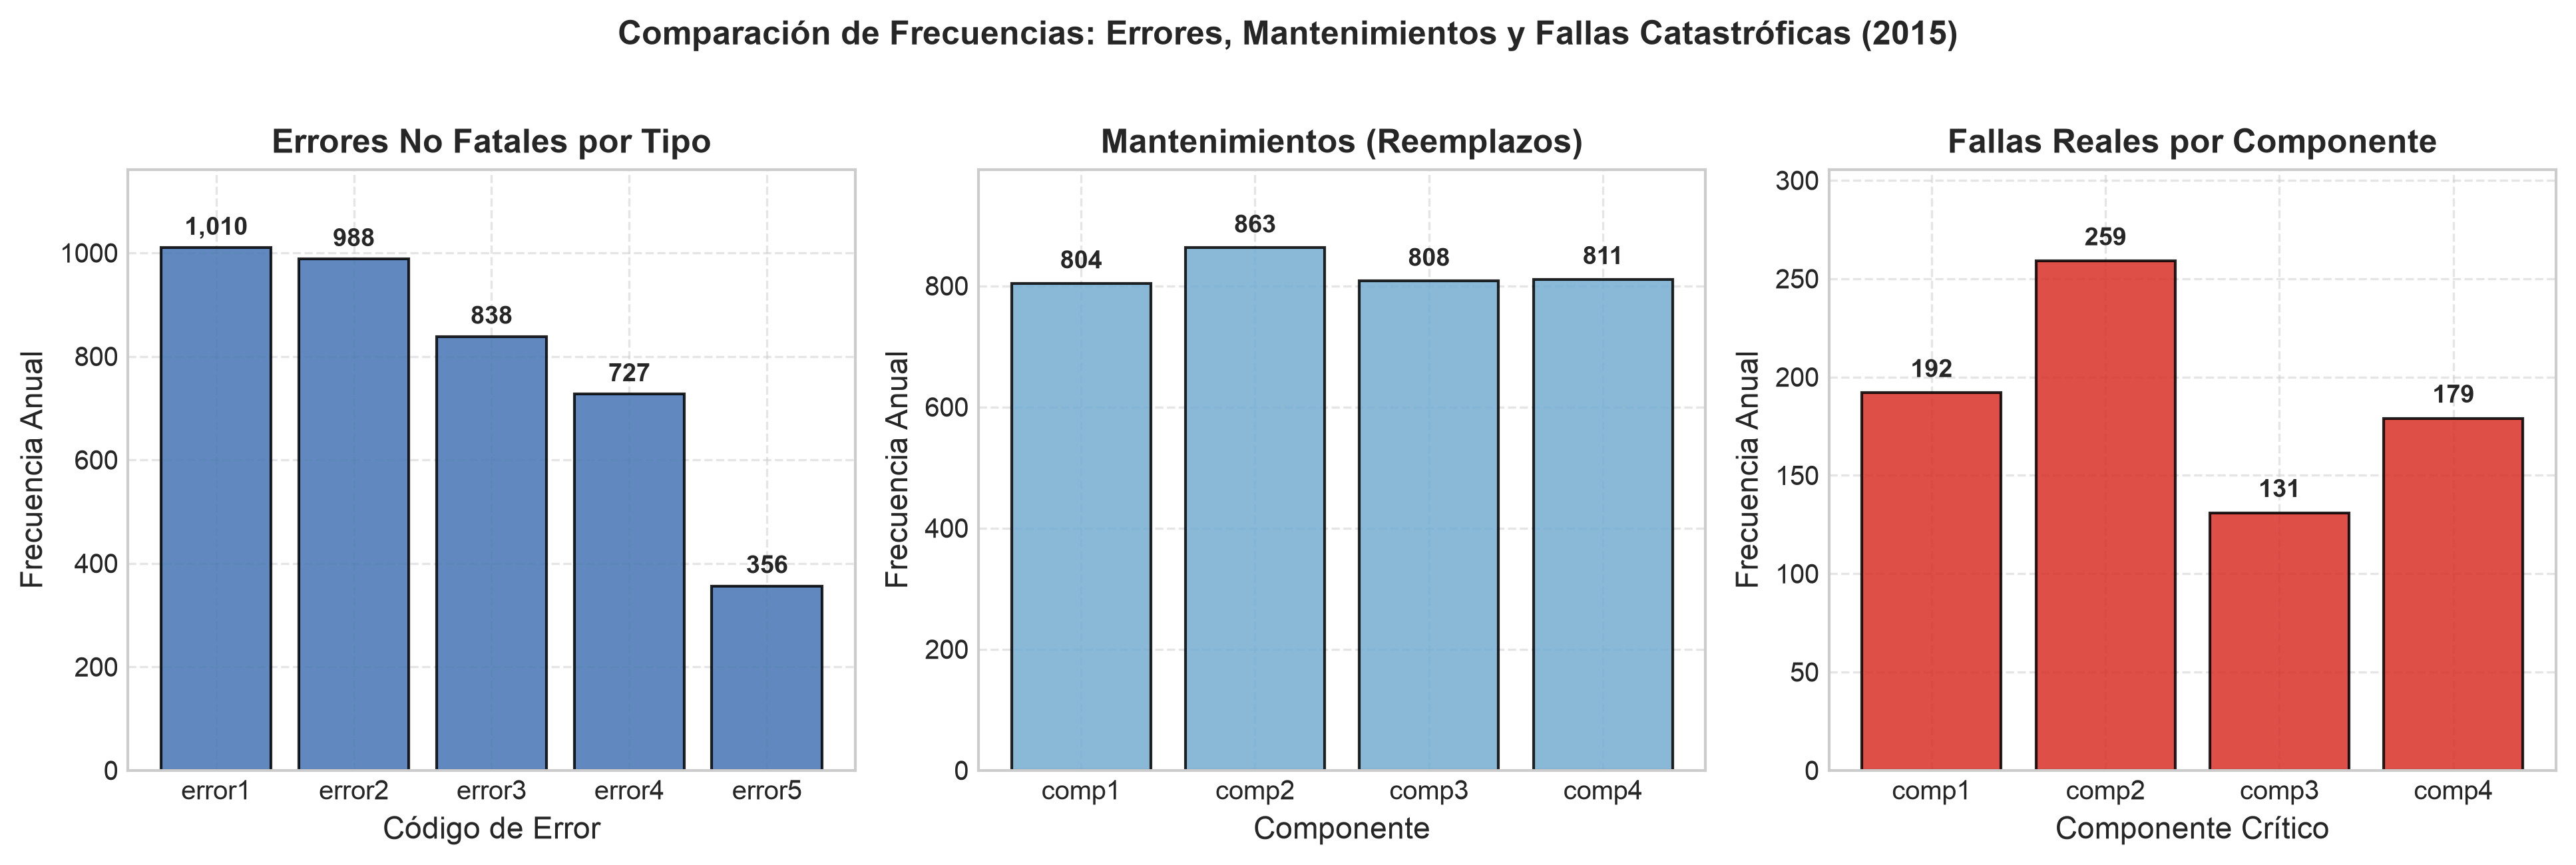
\includegraphics[width=\columnwidth]{../figures/fig2_frecuencia_eventos_desbalance.png}
\caption{Frecuencia anual de eventos: Errores no fatales (izq.), Mantenimientos (centro) y Fallas catastróficas por componente (der.).}
\label{fig:frecuencia_eventos}
\end{figure}

\subsection{Dinámica Temporal Previa al Colapso (48--72 Horas)}
Al aislar las 72 horas previas a cada colapso frente al régimen estacionario sano (Fig.~\ref{fig:telemetria_pre_falla}), emergen firmas de degradación unívocas para cada componente:
\begin{itemize}
    \item \textbf{Falla en comp1 (Eléctrico):} Desestabilización progresiva del voltaje con sobretensiones continuas que superan los 188 V en las últimas 24 horas.
    \item \textbf{Falla en comp2 (Hidráulico):} Sobrepresión severa en el circuito que escala hasta 128 psi en $t-12$ horas.
    \item \textbf{Falla en comp3 (Mecánico):} Pérdida drástica de velocidad rotacional que cae por debajo de 380 RPM debido a fricción anómala.
    \item \textbf{Falla en comp4 (Rodamientos):} Disparo exponencial de la vibración mecánica, superando 54 mm/s en las 24 horas precedentes.
\end{itemize}

\begin{figure*}[t]
\centering
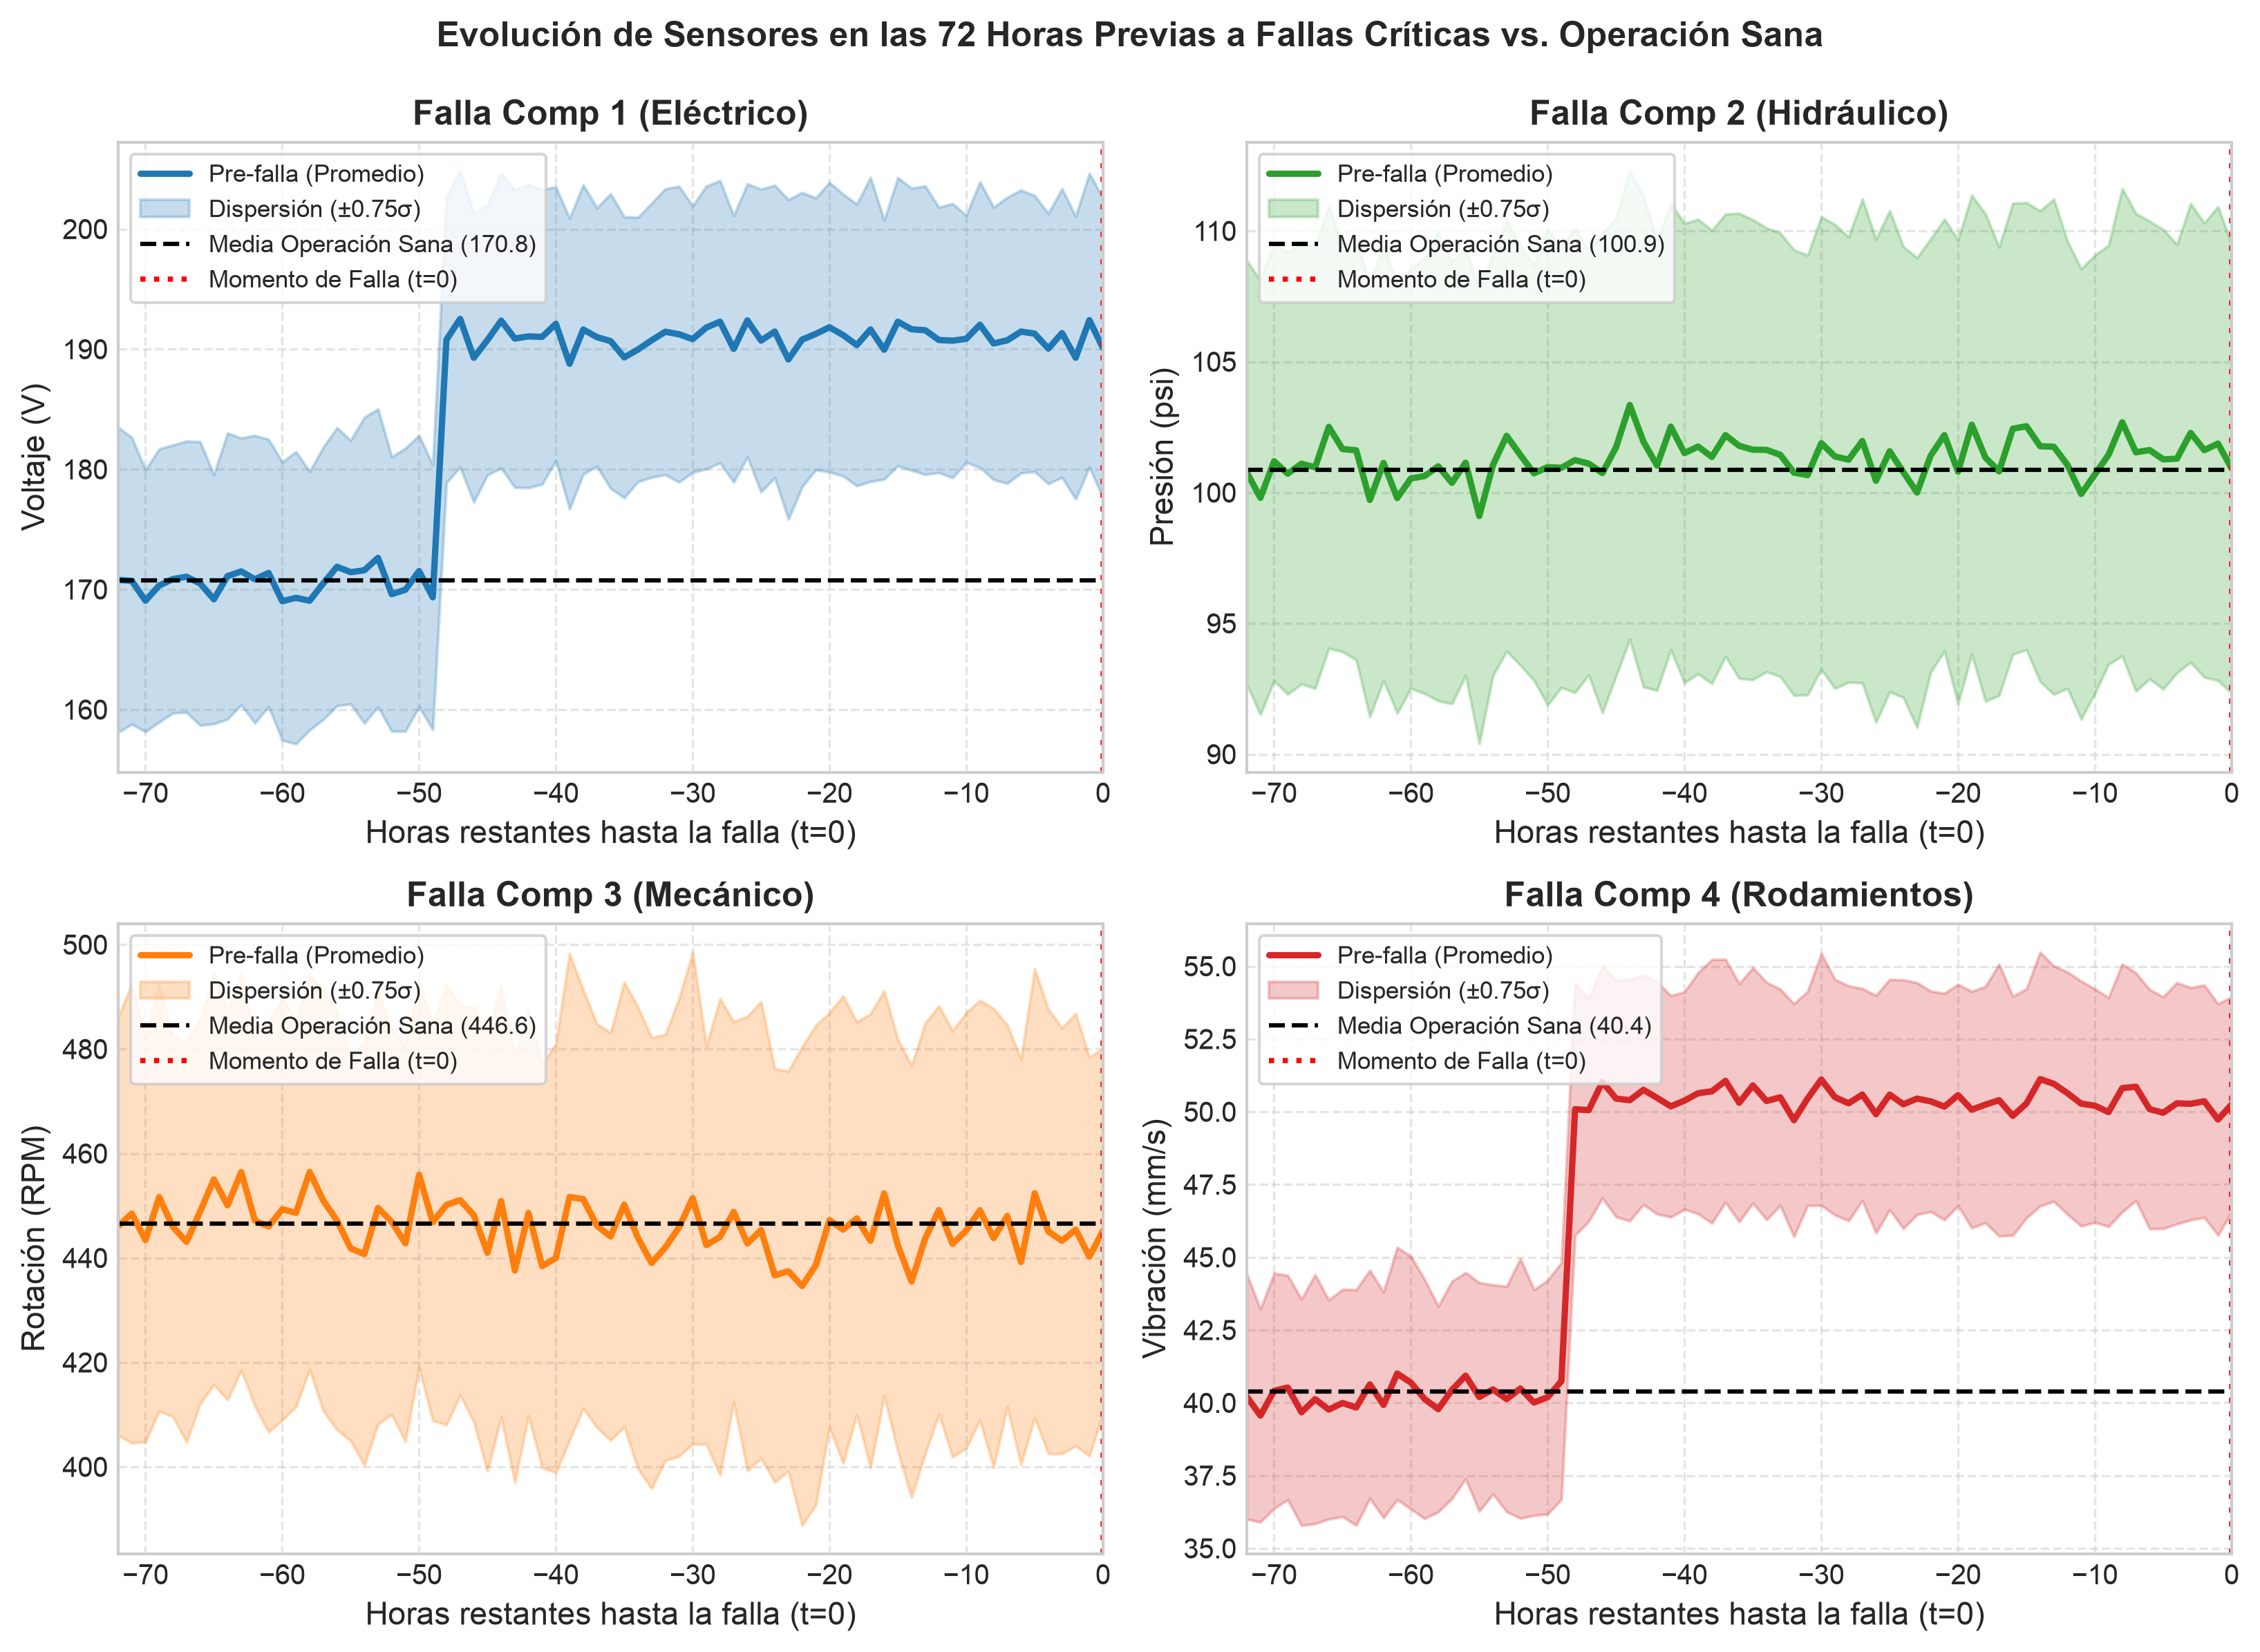
\includegraphics[width=0.95\textwidth]{../figures/fig3_telemetria_pre_falla_vs_sano.png}
\caption{Comportamiento dinámico de los cuatro sensores en las 72 horas previas a la falla de cada componente frente al promedio sano.}
\label{fig:telemetria_pre_falla}
\end{figure*}

\section{Definición de Etiquetas, Partición y Desbalance}
\subsection{Formulación Matemática de las Etiquetas}
Para cada máquina $m$ en cada instante horario $t$, el modelo recibe la historia causal observada hasta $t$ y resuelve:
\begin{enumerate}
    \item \textbf{Tarea Principal (Binaria):} Determinar la probabilidad de falla inminente en cualquier componente dentro del horizonte $(t, t+H]$ con $H=24$ horas:
    \begin{equation}
        y_{m,t}^{\text{bin}} = \mathbb{I} \left( \sum_{k=1}^4 \text{fallas}_{m,k}(t, t+24] > 0 \right)
    \end{equation}
    \item \textbf{Tarea Secundaria (Multiclase):} Identificar qué componente específico colapsará: $y_{m,t}^{\text{multi}} \in \{0: \text{Ninguno}, 1: \text{comp1}, \dots, 4: \text{comp4}\}$.
\end{enumerate}

\subsection{Partición Temporal Fija y Margen Anti-Fuga}
Para evitar fugas de información por autocorrelación temporal, se aplicó la partición temporal obligatoria:
\begin{itemize}
    \item \textbf{Entrenamiento:} 1 ene 2015 -- 31 ago 2015 (hasta 30 ago 23:00, $N = 580,200$).
    \item \textbf{Validación:} 1 sep 2015 -- 31 oct 2015 (hasta 30 oct 23:00, $N = 144,000$).
    \item \textbf{Prueba:} 1 nov 2015 -- 31 dic 2015 ($N = 144,000$, reservado y no tocado).
\end{itemize}
Se estableció un margen estricto de $H=24$ horas en las fronteras de corte para asegurar que ninguna etiqueta en entrenamiento observe fallas de septiembre y ninguna de validación observe fallas de noviembre.

\subsection{Tabla de Desbalance Extremo}
A pesar de que cada falla proyecta una ventana positiva de 24 horas, las horas en estado de alerta representan únicamente el \textbf{2.02\% en entrenamiento} y el \textbf{1.84\% en validación} (Tabla~\ref{tab:desbalance}). Este desbalance severo invalida el uso del \textit{Accuracy} como métrica guía, priorizando \textbf{PR-AUC} y el \textbf{Recall a Precisión fija $\ge 0.80$}.

\begin{table}[htbp]
\caption{Cuantificación del Desbalance de Clases (H = 24h)}
\label{tab:desbalance}
\centering
\begin{tabular}{lcrrrr}
\toprule
\textbf{Etiqueta / Componente} & \textbf{Clase} & \textbf{Train (N)} & \textbf{Train (\%)} & \textbf{Val (N)} & \textbf{Val (\%)} \\
\midrule
Ninguna Falla (Sano) & 0 & 568,458 & 97.98\% & 141,348 & 98.16\% \\
comp1 (Eléctrico) & 1 & 3,357 & 0.58\% & 498 & 0.35\% \\
comp2 (Hidráulico) & 2 & 3,849 & 0.66\% & 1,080 & 0.75\% \\
comp3 (Mecánico) & 3 & 2,001 & 0.34\% & 426 & 0.30\% \\
comp4 (Rodamientos) & 4 & 2,535 & 0.44\% & 648 & 0.45\% \\
\midrule
\textbf{TOTAL POSITIVOS (Bin.)} & 1--4 & \textbf{11,742} & \textbf{2.02\%} & \textbf{2,652} & \textbf{1.84\%} \\
\bottomrule
\end{tabular}
\end{table}

\section{Ingeniería de Variables y Mitigación de Fugas}
Se diseñó un vector de 31 características causales agrupadas en:
\begin{enumerate}
    \item \textbf{Estadísticas Móviles de Sensores (16 features):} Promedios y desviaciones estándar causales en ventanas cortas (3 h) y largas (24 h) sobre $[t-W+1, t]$ para cada sensor.
    \item \textbf{Frecuencia de Errores (6 features):} Conteo acumulado en las últimas 24 horas de cada error no fatal (\textit{error1} a \textit{error5}) y suma agregada (\textit{total\_errors\_24h}).
    \item \textbf{Desgaste Acumulado (4 features):} Horas transcurridas desde el último reemplazo previo de cada componente ($h\_since\_comp_k$).
    \item \textbf{Metadatos de Máquina (5 features):} Antigüedad en años (\textit{age}) y codificación one-hot del modelo (\textit{model1} a \textit{model4}).
\end{enumerate}

\textbf{Garantía Anti-Fuga en Escalamiento:} El escalador \texttt{StandardScaler} se ajustó (\textit{fit}) única y exclusivamente sobre los datos de entrenamiento (1 ene--30 ago). Las matrices de validación fueron normalizadas mediante inferencia ciega (\textit{transform}), evitando cualquier contaminación de distribuciones futuras.

\section{Resultados de la Línea Base Clásica}
Se entrenaron y evaluaron dos modelos bajo ponderación balanceada (\texttt{class\_weight='balanced'}):
\begin{enumerate}
    \item \textbf{Regresión Logística L2:} Modelo lineal de referencia ajustado sobre variables estandarizadas.
    \item \textbf{Gradient Boosting con Histogramas (HistGBDT):} Algoritmo no lineal basado en árboles de decisión optimizados con partición por histogramas (equivalente a LightGBM).
\end{enumerate}

\subsection{Métricas de Validación Binaria}
Como resume la Tabla~\ref{tab:resultados_baseline} y la Fig.~\ref{fig:curvas_pr_roc}, el modelo GBDT superó categóricamente a la Regresión Logística. En la curva Precision-Recall, GBDT alcanza un \textbf{PR-AUC de 0.9996} (frente a 0.8540 de la Regresión Logística). Bajo el umbral restrictivo de \textbf{Precisión $\ge 0.80$}, la Regresión Logística logra un Recall de 0.8179 en un umbral conservador de 0.9673, mientras que GBDT captura el \textbf{100\% de las fallas (Recall = 1.0000)} manteniendo una precisión superior al 80\%.

\begin{table}[htbp]
\caption{Desempeño Comparativo de Modelos de Línea Base en Validación}
\label{tab:resultados_baseline}
\centering
\begin{tabular}{lrrrr}
\toprule
\textbf{Modelo} & \textbf{PR-AUC} & \textbf{ROC-AUC} & \textbf{Rec (P$\ge$0.80)} & \textbf{Macro F1} \\
\midrule
Regresión Logística & 0.8540 & 0.9977 & 0.8179 & 0.8028 \\
\textbf{HistGBDT (Boosting)} & \textbf{0.9996} & \textbf{1.0000} & \textbf{1.0000} & \textbf{0.9960} \\
\bottomrule
\end{tabular}
\end{table}

\begin{figure}[htbp]
\centering
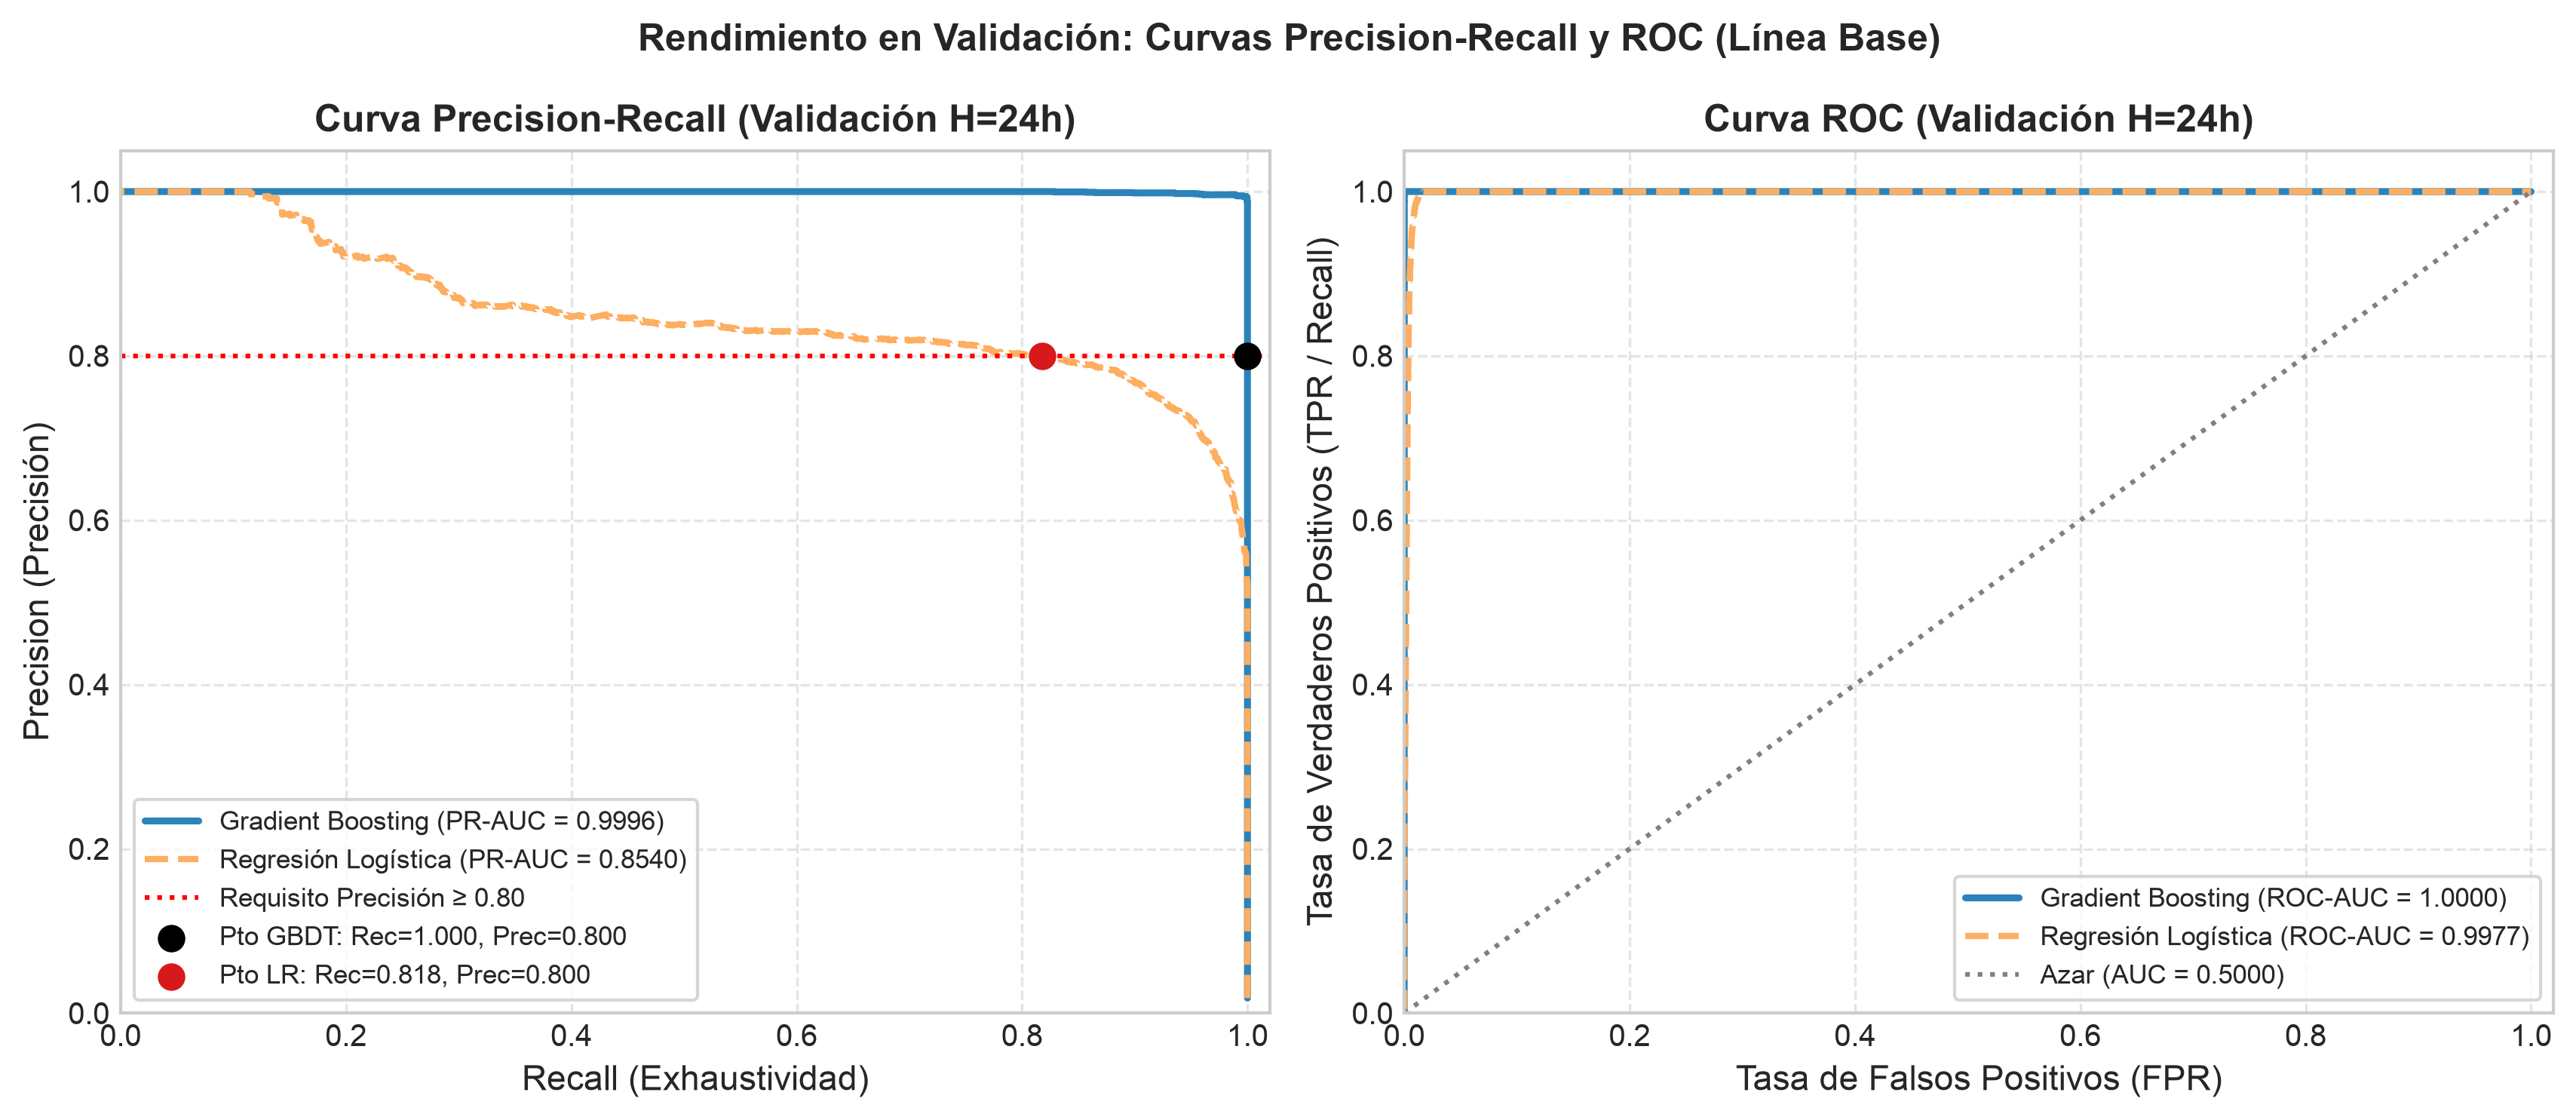
\includegraphics[width=\columnwidth]{../figures/fig4_curvas_pr_roc_validacion.png}
\caption{Curvas Precision-Recall (izq.) y ROC (der.) en el conjunto de validación ($H=24$h).}
\label{fig:curvas_pr_roc}
\end{figure}

\subsection{Matriz de Confusión Multiclase}
En la tarea de diagnóstico del componente crítico a fallar (Tabla~\ref{tab:metricas_multiclase} y Fig.~\ref{fig:matriz_confusion}), GBDT logró un \textbf{Macro F1 de 0.9960} con exactitud de 99.98\%. Para \textit{comp2} y \textit{comp3}, el modelo identificó el 100\% de los eventos sin una sola falsa alarma. Para \textit{comp1} alcanzó 100\% de recall con 98.03\% de precisión (10 falsas alarmas), y para \textit{comp4} capturó 643 de 648 eventos (99.23\% de recall con 98.77\% de precisión). En 141,348 horas sanas, el sistema generó únicamente 18 falsas alarmas en dos meses (~2 por semana en toda la flota de 100 máquinas).

\begin{table}[htbp]
\caption{Reporte Multiclase por Componente en Validación (HistGBDT)}
\label{tab:metricas_multiclase}
\centering
\begin{tabular}{lrrrr}
\toprule
\textbf{Componente} & \textbf{Precisión} & \textbf{Recall} & \textbf{F1-Score} & \textbf{Soporte} \\
\midrule
Ninguno (Sano) & 0.9999 & 0.9999 & 0.9999 & 141,348 \\
comp1 (Eléctrico) & 0.9803 & 1.0000 & 0.9901 & 498 \\
comp2 (Hidráulico) & 1.0000 & 1.0000 & 1.0000 & 1,080 \\
comp3 (Mecánico) & 1.0000 & 1.0000 & 1.0000 & 426 \\
comp4 (Rodamientos) & 0.9877 & 0.9923 & 0.9900 & 648 \\
\midrule
\textbf{Promedio Macro} & \textbf{0.9936} & \textbf{0.9984} & \textbf{0.9960} & \textbf{144,000} \\
\bottomrule
\end{tabular}
\end{table}

\begin{figure}[htbp]
\centering
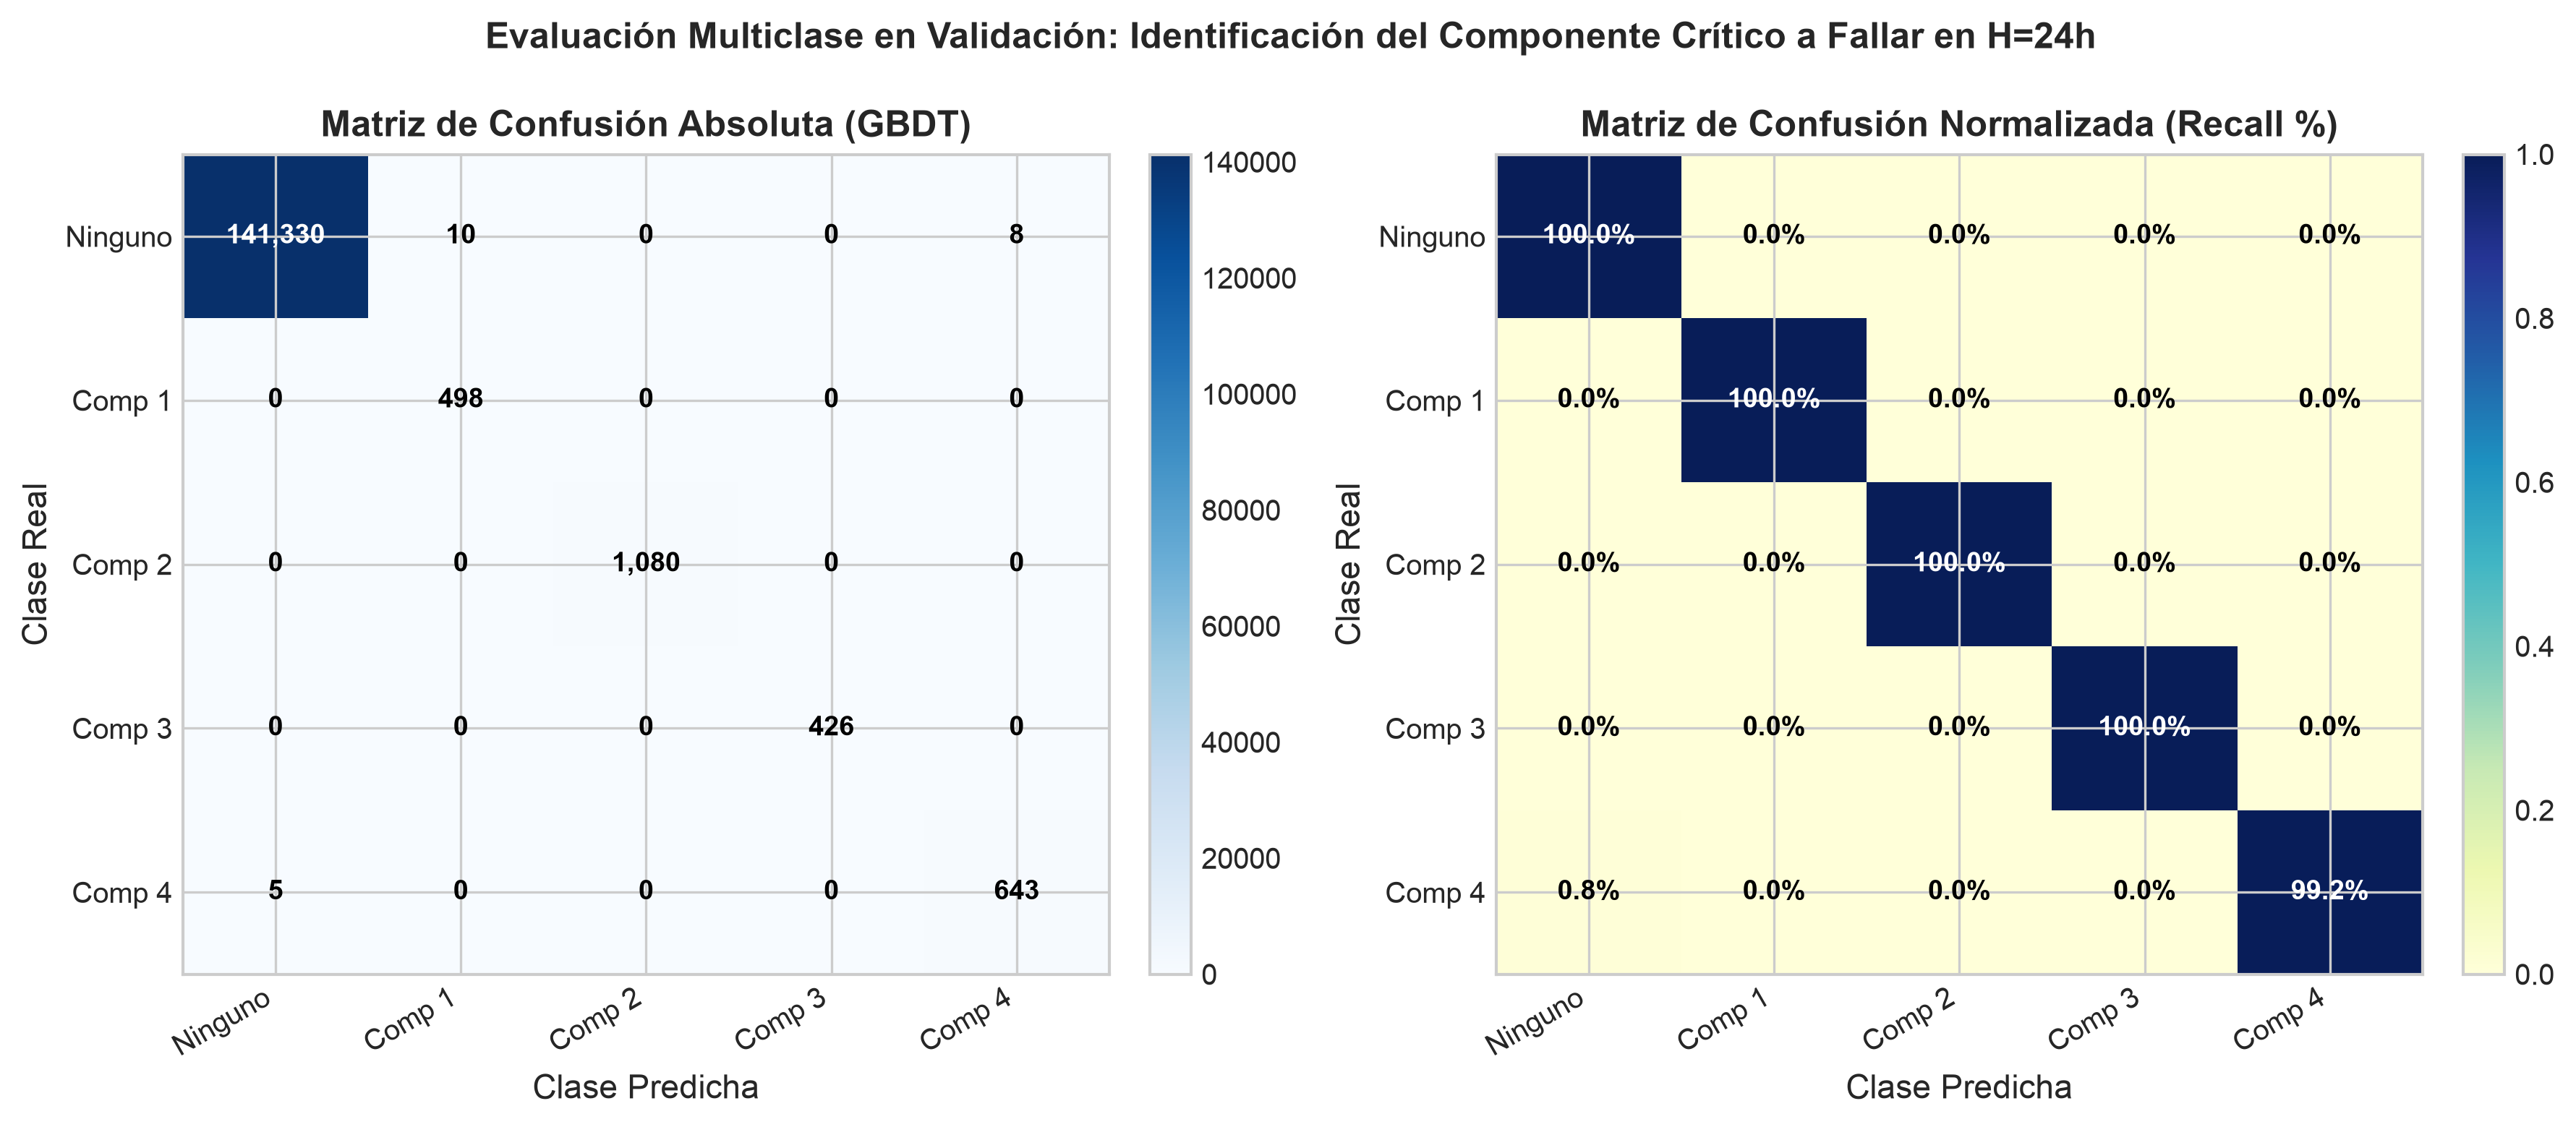
\includegraphics[width=\columnwidth]{../figures/fig5_matriz_confusion_multiclase.png}
\caption{Matriz de confusión multiclase en validación: conteos absolutos (izq.) y porcentajes de recall normalizados (der.).}
\label{fig:matriz_confusion}
\end{figure}

\section{Discusión y Conclusiones}
Los resultados de la Semana 1 confirman que la ingeniería de variables causales combinada con modelos de ensamble no lineales (\textit{HistGBDT}) constituye una línea base excepcionalmente robusta para la predicción de fallas industriales a 24 horas.

\textbf{Discusión Crítica sobre Datos Reales:} Aunque el desempeño en este dataset simulado es cuasi-perfecto, en una planta real se anticipan factores de perturbación severos: derivas no lineales de calibración en sensores, pérdida intermitente de paquetes por fallas de red IoT, y registros humanos de mantenimiento con desfasamiento temporal.

\textbf{Perspectiva hacia la Semana 2 (Deep Learning):} En la siguiente entrega se investigarán arquitecturas secuenciales profundas (LSTM/GRU bidireccional, convoluciones causales dilatadas TCN y transformadores temporales) sobre tensores multicanal ($L \in \{24, 72, 168\}$ horas) para determinar si las representaciones latentes superan las características manuales en anticipación y calibración.

\begin{thebibliography}{00}
\bibitem{b1} Microsoft Corporation, «Predictive Maintenance Modelling Guide,» \textit{Azure AI Gallery Documentation}, 2016.
\bibitem{b2} S. Hochreiter and J. Schmidhuber, «Long Short-Term Memory,» \textit{Neural Computation}, vol. 9, no. 8, pp. 1735--1780, 1997.
\bibitem{b3} S. Bai, J. Z. Kolter, and V. Koltun, «An Empirical Evaluation of Generic Convolutional and Recurrent Networks for Sequence Modeling,» \textit{arXiv:1803.01271}, 2018.
\bibitem{b4} T.-Y. Lin et al., «Focal Loss for Dense Object Detection,» \textit{IEEE ICCV}, pp. 2980--2988, 2017.
\end{thebibliography}

\end{document}
